\chapter{Pràctica}
\section{Placa base CC1352R1}
Per analitzar el protocol BLE i veure les seves característiques s'ha utilitzat el kit per desenvolupament ràpid del microcontrolador CC1352R1.
\begin{figure}[h!]
	\begin{center}
		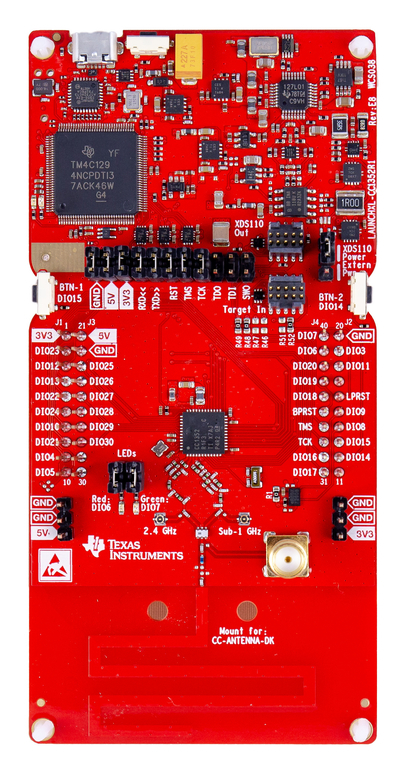
\includegraphics[width=0.8\textwidth]{./images/launchxl-cc1352r1.jpg}
		\caption{Placa \cite{placa}}
	\end{center}
\end{figure}

Aquesta placa permet el desenvolupament d'aplicacions en BLE utilitzant el microcontrolador CC1352 de Texas Instruments.
La placa té les següents característiques:


\section{Software}
Per al desenvolupament de projectes per a la placa s'ha utilitzat el entorn de desenvolupament Code Composer Studio. El software de desenvolupament és el SimpleLink(TM) CC13X2
Comentar tema versió

\section{Project 0}
El Project 0 és el projecte instal·lat amb que les plaques vénen de fàbrica. Aquest projecte exposa certs serveis a través de BLE i et permet veure una comunicació simple entre la placa i un dispositiu mòbil. La comunicació es fa a través del control dels dos LEDs que te la placa (els LEDs que estan directament controlars pel microcontrolador) i també per l'estat dels botons que hi ha a ambdós costats de la placa.
*Aquest projecte també inclou altres serveis en que no entrarem.



\section{Coses per defecte}
\subsection{Fórmules, figures i taules}

\subsubsection{Fórmules}

Pel que fa al format de les formules, no cal fer absolutament res. \LaTeX \ ja ho fa tot per vosaltres :-)  

Simplement el que heu de fer és escriure la fórmula com per exemple:

\begin{equation}\label{E:prova}
\sum _{i=0}^{N} \sum _{j=0}^{N} \frac{\lambda _{ij}}{\alpha _i \beta_ j} \cdot \cos (2\pi f_i) \sin(2 \pi f_j)
\end{equation}

i per citar-la és tant fàcil com fer: \ref{E:prova}

\subsubsection{Figures}

Pel que fa al format de les figures, no cal fer absolutament res. \LaTeX \ ja ho fa tot per vosaltres :-) . 

Simplement el que heu de fer és inserir la figura amb el codi següent:

\begin{verbatim}
\begin{figure}[htb]
\begin{center}
\includegraphics[width=0.5\textwidth]{./setup/EETAC-positiu-negre}
\caption{Exemple de figura}
\label{F:prova}
\end{center}
\end{figure}
\end{verbatim}

donant com a resultat la figura \ref{F:prova}.

\begin{figure}[htb]
\begin{center}
\includegraphics[width=0.5\textwidth]{./setup/EETAC-positiu-negre}
\caption{Exemple de figura}
\label{F:prova}
\end{center}
\end{figure}

Podem tocar la variable \texttt{width} per ajustar l'amplada de la figura com més ens convingui. Teniu en compte que la variable \texttt{textwidth} guarda el valor de l'amplada del texte dins la pàgina i per tant és una bona referència per delimitar amplades de figura, així doncs, la figura \ref{F:prova} ocupa la meitat de l'amplada del texte en una pàgina. 

Podeu arranjar múltiples imatges en una sola figura amb el paquet \texttt{subfigmat}, que defineix un nou entorn \texttt{subfigmatrix} que accepta per argument el nombre de columnes del arranjament. Per exemple, per fer una figura amb tres columnes d'imatges:

\begin{verbatim}
\begin{figure}[htb]
  \begin{center}
    \begin{subfigmatrix}{3}
      \subfigure[Títol subfigura 1]
         {\includegraphics{./setup/EETAC-positiu-negre}\label{SF:S1}} 
      \subfigure[Títol subfigura 2]
         {\includegraphics{./setup/EETAC-positiu-negre}\label{SF:S2}} 
      \subfigure[Títol subfigura 3]
         {\includegraphics{./setup/EETAC-positiu-negre}\label{SF:S3}} 
      \subfigure[Títol subfigura 4]
         {\includegraphics{./setup/EETAC-positiu-negre}\label{SF:S4}} 
      \subfigure[Títol subfigura 5]
         {\includegraphics{./setup/EETAC-positiu-negre}\label{SF:S5}} 
      \subfigure[Títol subfigura 6]
         {\includegraphics{./setup/EETAC-positiu-negre}\label{SF:S6}} 
    \end{subfigmatrix}
    \caption{Exemple d'arranjament amb múltiples imatges}
    \label{F:prova2}
  \end{center}
\end{figure}
\end{verbatim}

que dona com a resultat, la figura \ref{F:prova2}.

\begin{figure}[htb]
  \begin{center}
    \begin{subfigmatrix}{3}
      \subfigure[Títol subfigura 1]{\includegraphics{./setup/EETAC-positiu-negre}\label{SF:S1}} 
      \subfigure[Títol subfigura 2]{\includegraphics{./setup/EETAC-positiu-negre}\label{SF:S2}} 
      \subfigure[Títol subfigura 3]{\includegraphics{./setup/EETAC-positiu-negre}\label{SF:S3}} 
      \subfigure[Títol subfigura 4]{\includegraphics{./setup/EETAC-positiu-negre}\label{SF:S4}} 
      \subfigure[Títol subfigura 5]{\includegraphics{./setup/EETAC-positiu-negre}\label{SF:S5}} 
      \subfigure[Títol subfigura 6]{\includegraphics{./setup/EETAC-positiu-negre}\label{SF:S6}} 
    \end{subfigmatrix}
    \caption{Exemple d'arranjament amb múltiples imatges}
    \label{F:prova2}
  \end{center}
\end{figure}

%%%%%%%%%%%%%%%%%%%%%%%%%%%%%%%%%%%%%%%%%%%%%%%%%%%%%%%%%%%%%%%%%%%%%%%%%%%%%%


\subsubsection{Taules}

Pel que fa a la numeració de les taules, no cal fer gran cosa. \LaTeX \ ja fa gran part de la feina bruta. 

Simplement el que heu de fer és inserir la figura amb el codi següent:

\begin{verbatim}
\begin{table}[htb]
\begin{center}
\begin{tabular}{|c|l|r|}
\hline
{\bf Títol de la Columna 1} & {\bf Títol de la Columna 2} & 
{\bf Títol de la Columna 3}  \\ \hline \hline
centrada        & a l'esquerra    & a la dreta       \\ \hline
centrada        & a l'esquerra    & a la dreta       \\ \hline
centrada        & a l'esquerra    & a la dreta       \\ \hline
centrada        & a l'esquerra    & a la dreta       \\ \hline
centrada        & a l'esquerra    & a la dreta       \\ \hline
\end{tabular}
\caption{Exemple de taula}
\label{T:prova}
\end{center}
\end{table}
\end{verbatim}

donant com a resultat la taula \ref{T:prova}.


\begin{table}[htb]
\caption{Exemple de taula}
\begin{center}
\begin{tabular}{|c|l|r|}
\hline
{\bf Títol de la Columna 1} & {\bf Títol de la Columna 2} & {\bf Títol de la Columna 3}  \\ \hline \hline
centrada        & a l'esquerra    & a la dreta       \\ \hline
centrada        & a l'esquerra    & a la dreta       \\ \hline
centrada        & a l'esquerra    & a la dreta       \\ \hline
centrada        & a l'esquerra    & a la dreta       \\ \hline
centrada        & a l'esquerra    & a la dreta       \\ \hline
\end{tabular}
\label{T:prova}
\end{center}
\end{table}

L'entorn \texttt{tabular} que ofereix \LaTeX \ és molt complet i permet crear multitud de taules diferents, tot i que és alhora bastant complexe. Cau fora de les intencions del present document descriure la sintaxis i el format d'aquest tipus d'entorn. És molt fàcil trobar informació al respecte amb llibres especialitzats o simplement a Internet. 


\subsection{Estudi d'ambientalització}

En general l'estudi d'ambientalització es podrà incloure dins de la introducció o a les conclusions, llevat del cas que les repercussions ambientals del treball tinguin una importància tant rellevant que sigui recomanable dedicar-hi un capítol específic.


\subsection{Bibliografia}

Tret que el treball consisteixi en la cerca de bibliografia sobre un tema concret, la bibliografia ha de contenir només la llista d'obres consultades.

A la bibliografia s'han de llistar conjuntament llibres i articles de revistes. Citar una referència bibliogràfica és tant fàcil com fer:

\begin{verbatim}
\cite{prova1}
\end{verbatim}

per citar la referència \cite{prova1}.

El format de la bibliografia es genera automàticament. Un altre (gran!) avantatge del \LaTeX \ :-)


\section{Apèndixs}

En general, cal posar als apèndixs totes les dades i documents que farien el text feixuc i dificultarien la seva lectura, sense oblidar que les contínues referències als apèndixs poden obligar al lector a interrompre constantment la lectura del treball. És per això, que els apèndixs poden incloure diagrames, dades estadístiques, taules de resultats i desenvolupaments teòrics complementaris.

En el cas que, amb el conjunt d'apèndixs, el treball tingui una extensió superior als 100 fulls (aproximadament 200 pàgines), els apèndixs s'han de enquadernar en un volum separat del cos principal del treball. Aquesta plantilla ja proporciona les eines necessàries per fer la portada necessària en cas d'enquadernar els apèndixs per separat.
